\documentclass{standalone}
\usepackage{ tikz }
\usepackage{ xparse }
\usepackage{ amssymb }
\input{macros/all}

\begin{document}
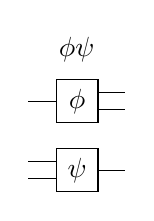
\begin{tikzpicture}[yscale=-1,x=1em,y=1.25em]

    \node at (12.75, -2.5) {$\phi \tensor \psi$};

    \node[draw, minimum height = 1.5em, minimum width = 1.5em, anchor = west] at (12,-1){$\phi$};
    \node[draw, minimum height = 1.5em, minimum width = 1.5em, anchor = west] at (12,1){$\psi$};

    \draw (12,-1) -- (11,-1);
    \draw (12,0.75) -- (11,0.75);
    \draw (12,1.25) -- (11,1.25);

    \draw (13.5,-0.75) -- (14.5, -0.75);
    \draw (13.5,-1.25) -- (14.5, -1.25);
    \draw (13.5,1) -- (14.5, 1);

\end{tikzpicture}
\end{document}